% =============================================================================
% Informe Técnico Final: USS SpiderBot — Robot Cuadrúpedo de Reconocimiento
% Taller de Programación I, Universidad San Sebastián. Año 2026.
% Compilar con: xelatex informe_proyecto_spiderbot.tex
% =============================================================================
\documentclass[12pt]{article}

% --- Paquetes Básicos ---
\usepackage{fontspec}
\usepackage[spanish,es-noshorthands,es-noquoting]{babel}
\usepackage{geometry}
\geometry{a4paper, margin=2.5cm} % Márgenes estándar según norma USS
\usepackage{setspace}
\setstretch{1.5} % Interlineado 1.5 según norma USS
\usepackage{graphicx}
\usepackage{booktabs}  % Para tablas formato APA
\usepackage{tabularx}

% --- Paquetes Matemáticos y de Símbolos ---
\usepackage{amsmath}   % Esencial para fórmulas avanzadas
\usepackage{amssymb}   % Para símbolos
\usepackage{textcomp}  % Para manejar símbolos de texto

% --- Paquetes de Formato y Enlaces ---
\usepackage{hyperref}  
\hypersetup{
    colorlinks=true,   % True: colorea el texto del link
    urlcolor=blue,     % Color para los enlaces web externos (formato APA estándar)
    linkcolor=black,   % Color para los enlaces internos (como el índice)
    citecolor=black    % Color para las citas bibliográficas
}
\usepackage{titlesec}
\usepackage{xcolor}
\usepackage{xurl} % Permite romper las URLs en cualquier carácter
\usepackage{listings}

% --- Configuración de Títulos ---
\titleformat{\section}{\normalfont\Large\bfseries}{\thesection}{1em}{}
\titleformat{\subsection}{\normalfont\large\bfseries}{\thesubsection}{1em}{}
\titleformat{\subsubsection}{\normalfont\normalsize\bfseries}{\thesubsubsection}{1em}{}

\newcommand{\codigo}[1]{\texttt{#1}}

\begin{document}

% ======================================================
% PORTADA
% ======================================================
\begin{titlepage}
    \centering
    {\bfseries\LARGE Universidad San Sebastián \par}
    \vspace{1cm}
    
\includegraphics[width=0.4\textwidth]{logo_uss.png} \\
    \vspace{1cm}
    {\scshape\Large Facultad de Ingeniería y Tecnología \par}
    {\large Carrera de Ingeniería Civil Informática \par}
    \vspace{1.5cm}
    {\bfseries\huge Informe Técnico Final: \par}
    {\Large USS SpiderBot --- Robot Cuadrúpedo de Reconocimiento \par}
    \vspace{2cm}
    
    {\large \textbf{Integrantes y Roles:} \par}
    \begin{tabular}{ll}
        Moisés Amundarain & Integración y Firmware Asíncrono \\
        Camila Aravena & Diseño 3D en OpenSCAD y Tolerancias \\
        Fernando Ramírez & Configuración Electrónica y Potencia \\
        Juan Pablo Vargas & Simulación Wokwi y Calibración IMU \\
        María José Santander & Dashboard Web Embebido e Interfaz SVG \\
    \end{tabular}
    \vfill
    {\large Puerto Montt, Chile \par}
    {\large 1 de Julio de 2026 \par}
\end{titlepage}

% ======================================================
% ÍNDICE
% ======================================================
\newpage
\tableofcontents
\newpage

% ======================================================
% 1. IDENTIFICACIÓN DEL GRUPO
% ======================================================
\section{Identificación del Grupo}
\begin{table}[h!]
\centering
\begin{tabular}{p{5cm}p{10cm}}
\toprule
\textbf{Parámetro} & \textbf{Detalle} \\
\midrule
Asignatura & Taller de Programación I \\
Evaluación & Solemne 3 \\
Microcontrolador & ESP32 DevKit V1 \\
Lenguaje & MicroPython (v1.20+) \\
Integrante 1 & Moisés Amundarain — [Integración y Firmware Asíncrono] \\
Integrante 2 & Camila Aravena — [Diseño 3D en OpenSCAD y Tolerancias] \\
Integrante 3 & Fernando Ramírez — [Configuración Electrónica y Potencia] \\
Integrante 4 & Juan Pablo Vargas — [Simulación Wokwi y Calibración IMU] \\
Integrante 5 & María José Santander — [Dashboard Web Embebido e Interfaz SVG] \\
Fecha & 1 de Julio de 2026 \\
\bottomrule
\end{tabular}
\end{table}

% ======================================================
% 2. DESCRIPCIÓN DEL SISTEMA
% ======================================================
\section{Descripción del Sistema}
El proyecto \textbf{USS SpiderBot} consiste en el diseño, modelado mecánico, desarrollo de hardware y arquitectura de software de un robot caminador cuadrúpedo de 4 grados de libertad (4-DoF) con rodillas rígidas. El sistema ha sido diseñado específicamente para la exploración autónoma o asistida y el reconocimiento de entornos hostiles o zonas de desastre colapsadas por escombros, donde la locomoción tradicional por ruedas u orugas resulta ineficaz.

El robot opera de manera asíncrona mediante un firmware multitarea cooperativo no bloqueante que corre sobre una placa ESP32 DevKit V1. Implementa una marcha secuencial de gateo oscilante de caderas (Crawl Gait) y utiliza un sensor inercial inteligente para identificar inestabilidades, caídas dinámicas y empujones externos en tiempo real, garantizando la detección autónoma de accidentes en campo. Adicionalmente, cuenta con evasión reactiva de obstáculos frontal por sensor ultrasónico y expone un servidor HTTP nativo con un Dashboard web interactivo para telemetría vectorial y mando manual.

\subsection{Funciones principales que cumple el sistema:}
\begin{itemize}
    \item \textbf{Monitoreo Inercial Continuo:} Medición de los ángulos de inclinación (Pitch y Roll) mediante la IMU MPU6050 a una frecuencia de refresco de $20\text{ Hz}$.
    \item \textbf{Clasificación de Inteligencia Artificial Sensorial:} Monitoreo y diagnóstico local de inestabilidades dinámicas, caídas físicas (failsafe automático) y empujones externos mediante un árbol de decisión embebido.
    \item \textbf{Locomoción Secuencial Estable (Crawl Gait):} Desplazamiento del cuerpo manteniendo en todo momento al menos tres extremidades en contacto para asegurar que el centro de masa resida dentro del polígono de sustentación.
    \item \textbf{Evasión Reactiva de Obstáculos:} Detección de proximidad frontal mediante sensor HC-SR04. Ante lecturas inferiores a $15\text{ cm}$, se cancela de forma inmediata la locomoción ($<25\text{ ms}$), se activa una alarma sonora mediante el buzzer y se retorna a pose segura.
    \item \textbf{Control y Telemetría Remota Web:} Servidor web asíncrono que expone una consola de control remota en CSS Glassmorphism y JS nativo, con actualización de telemetría y renderizado vectorial de inclinación SVG.
\end{itemize}

\newpage

% ======================================================
% 3. DISEÑO MECÁNICO Y ESTRUCTURAL (OPENSCAD)
% ======================================================
\section{Diseño Mecánico y Estructural (OpenSCAD)}
El modelado tridimensional de las piezas se realizó de forma paramétrica en OpenSCAD utilizando el paradigma de geometría sólida constructiva (CSG).

\subsection{Estructura del Chasis (Doble Deck)}
El cuerpo central del robot consta de un sistema de doble placa circular (doble deck) que aísla los componentes de potencia y cableado del plano de los sensores y control:
\begin{itemize}
    \item \textbf{Placa Inferior:} Cilindro plano de radio $r = 65\text{ mm}$ y espesor $t = 3\text{ mm}$ que aloja perimetralmente los 4 brackets de fijación de servos de cadera. Cuenta con ranuras pasantes para la fijación de la batería mediante correas de velcro.
    \item \textbf{Placa Superior:} Placa de protección que se acopla a la inferior mediante 4 pilares espaciadores M3 de $19\text{ mm}$ de alto. Incorpora una cuna central de dimensiones $84\text{ x }56\text{ x }3\text{ mm}$ para alojar a presión la protoboard de 400 puntos, una cuna trasera para el regulador XL6009E1 y 4 agujeros de $14\text{ mm}$ de diámetro para el ruteo de cables.
    \item \textbf{Soporte HC-SR04:} Soporte vertical de $2\text{ mm}$ de espesor con dos orificios de $16.5\text{ mm}$ de diámetro espaciados a $26\text{ mm}$ entre centros, reforzado por dos gussets triangulares laterales para resistir fuerzas de cizalladura inerciales en caso de impacto.
\end{itemize}

\begin{figure}[htbp]
    \centering
    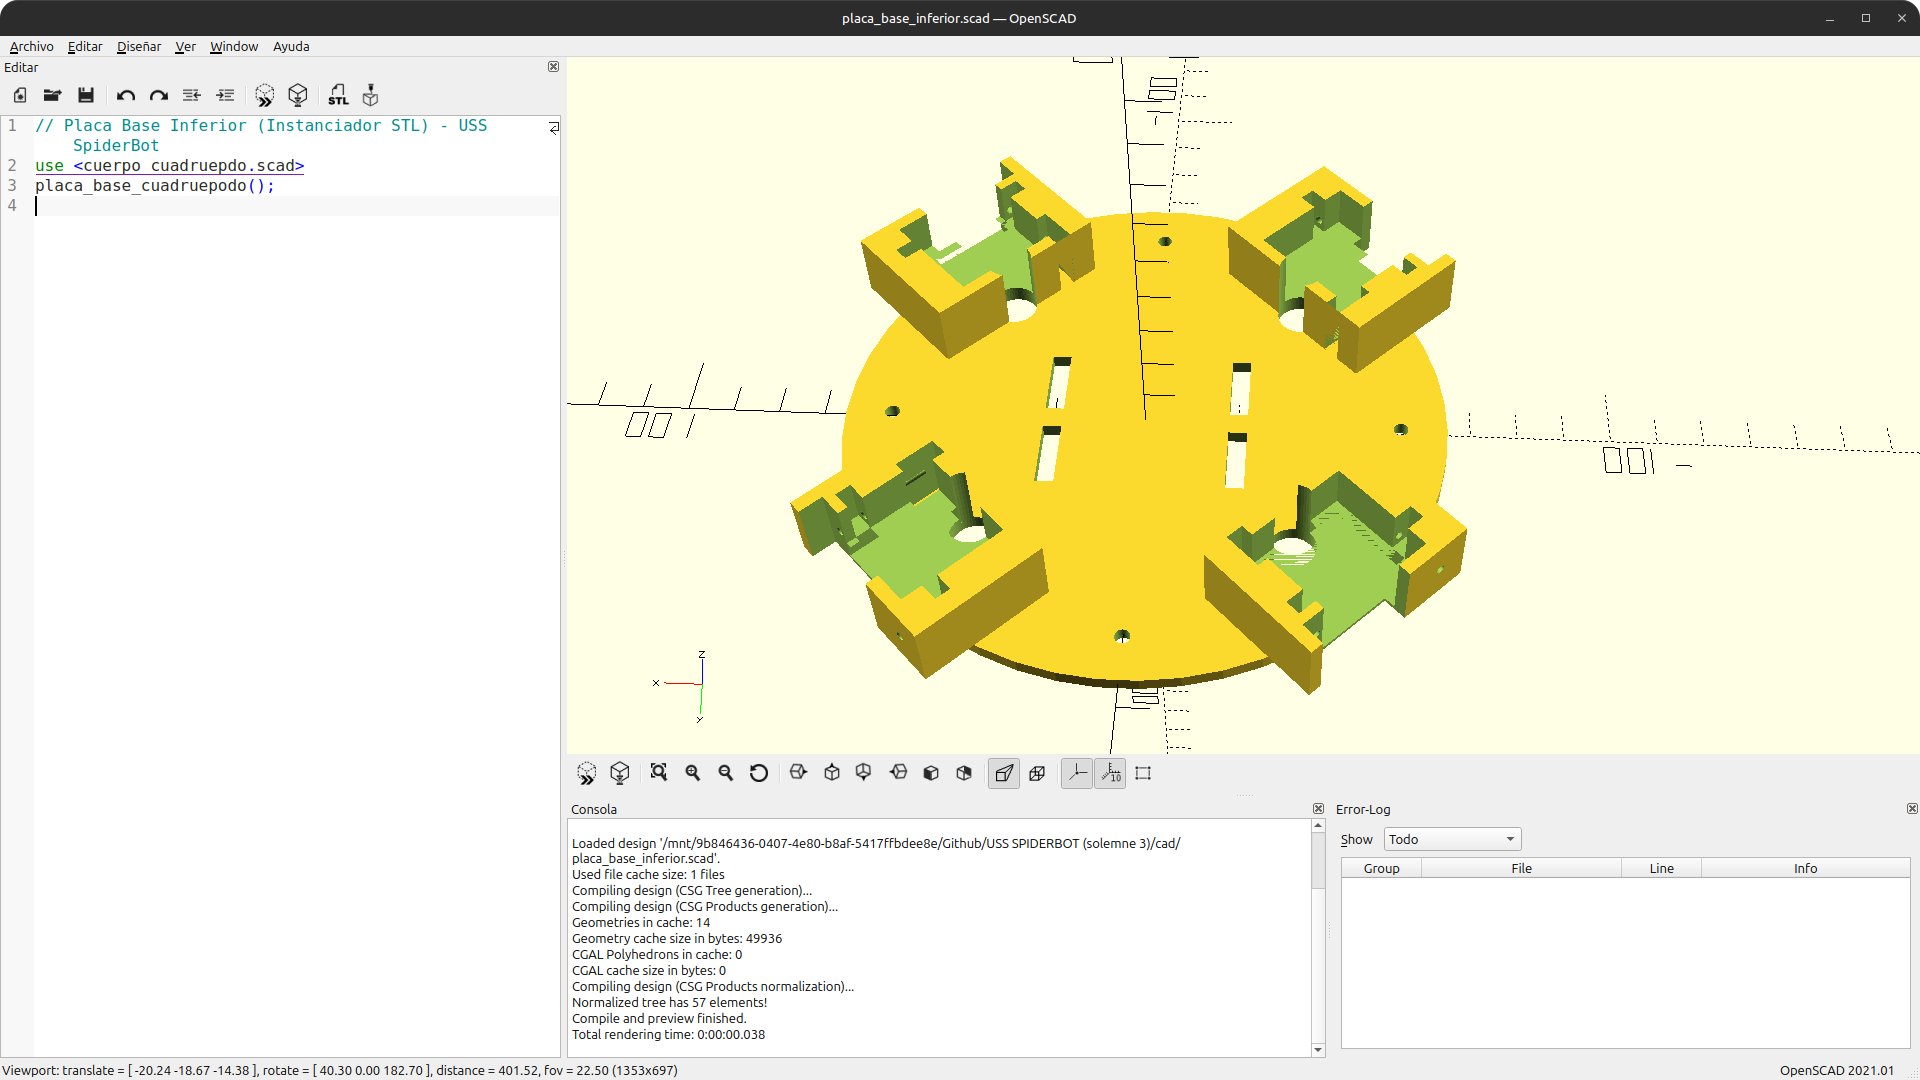
\includegraphics[width=0.45\textwidth]{Captura de pantalla de 2026-06-28 18-10-53.png}
    \hfill
    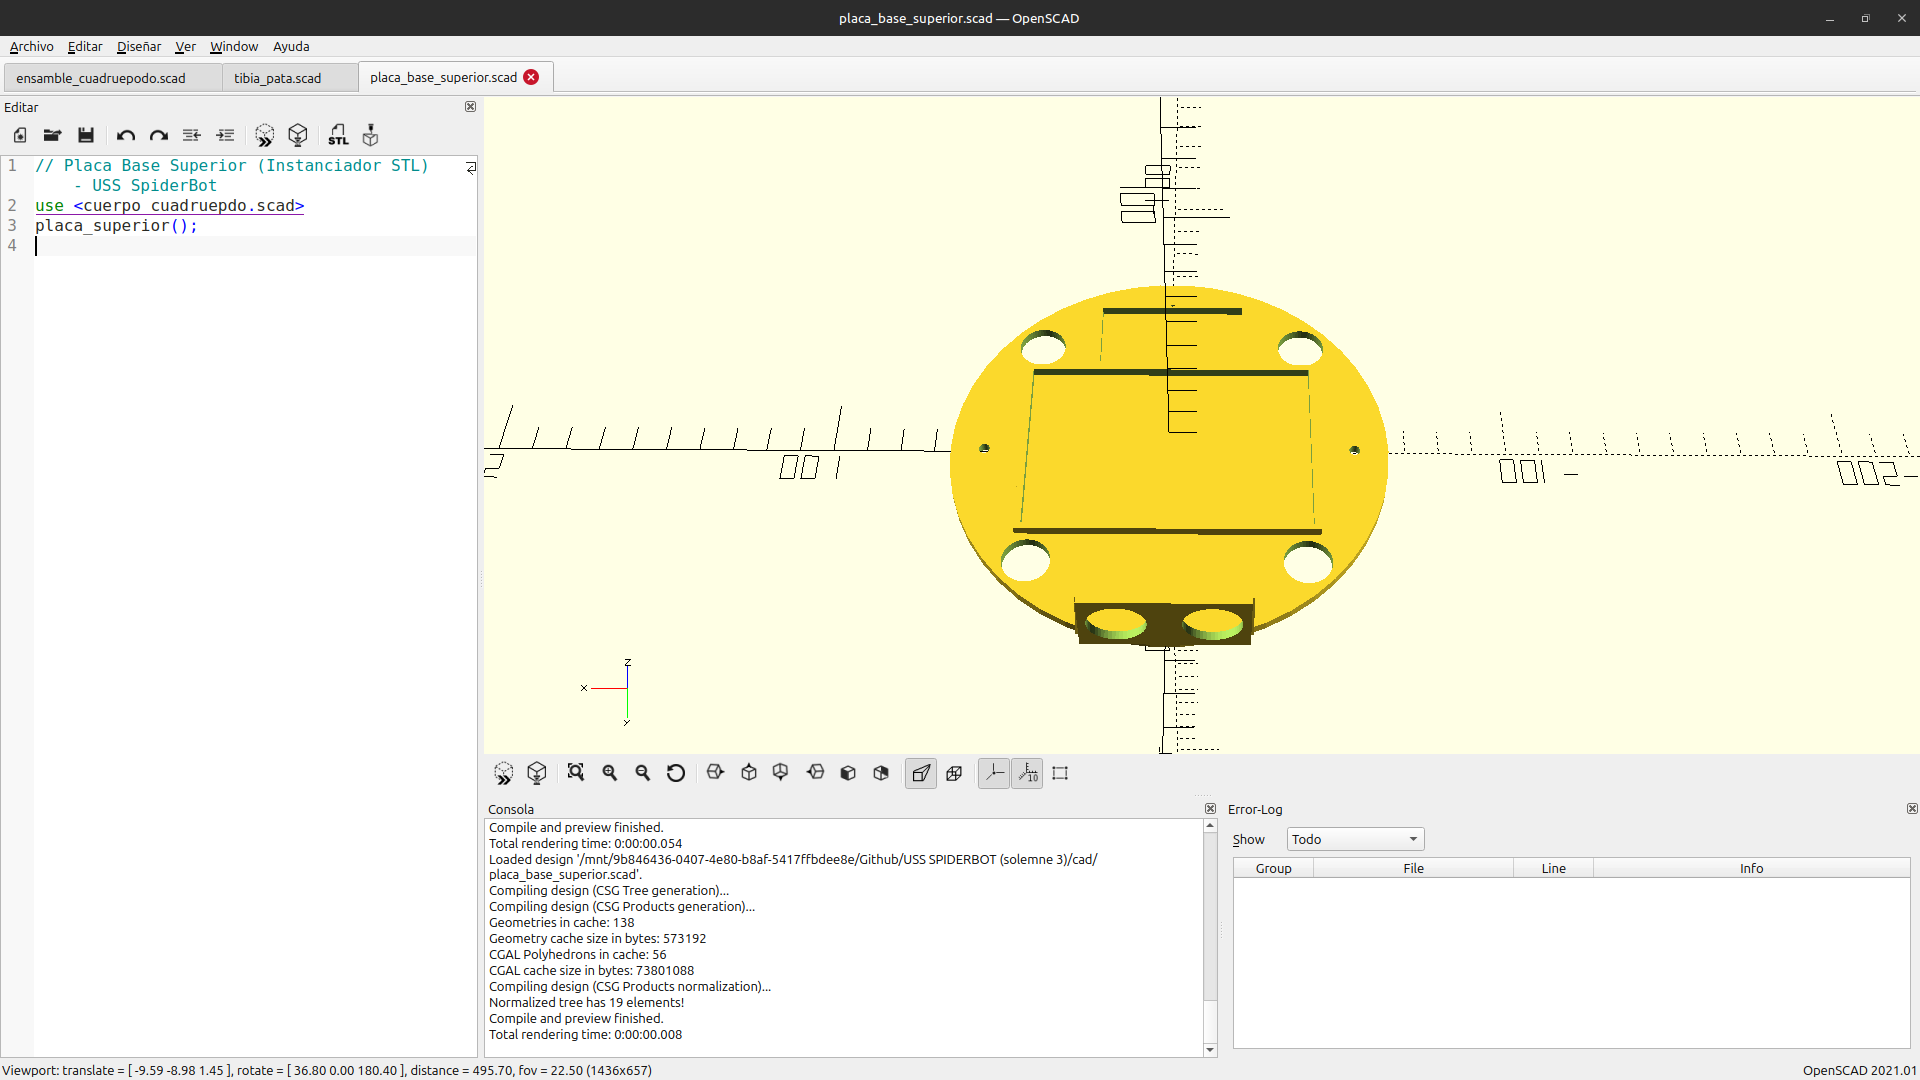
\includegraphics[width=0.45\textwidth]{openscad_screenshot_4.png}
    \caption{Modelado paramétrico en OpenSCAD de la placa base inferior (izquierda) y placa base superior (derecha).}
    \label{fig:placas_chasis}
\end{figure}

\begin{figure}[htbp]
    \centering
    
\includegraphics[width=0.55\textwidth]{spiderbot_render.png}
    \caption{Renderizado 3D paramétrico del chasis final y las extremidades articuladas del USS SpiderBot.}
    \label{fig:spiderbot_render}
\end{figure}

\subsection{Articulaciones y Extremidades (Fémur y Tibia)}
La configuración de 4-DoF del robot simplifica las extremidades eliminando el servomotor de rodilla. Las uniones fémur-tibia están bloqueadas rígidamente a 90 grados, reduciendo la masa móvil y el número de cables.
\begin{itemize}
    \item \textbf{Fémur:} Brazo de articulación de $55\text{ mm}$ de longitud entre centros. Une la corona del servo de cadera con la tibia de forma rígida. Se utilizó la función \codigo{hull()} para conectar suavemente la corona cilíndrica con la cavidad prismática del servo de rodilla (bloqueado), optimizando la distribución de masa y la resistencia a la flexión.
    \item \textbf{Tibia:} Pierna inferior curva con una longitud vertical de $65\text{ mm}$ y pie semiesférico de radio $r = 5.5\text{ mm}$. La curvatura estructural del modelo aumenta el despeje libre sobre el suelo y distribuye las fuerzas de reacción del impacto del pie en la marcha.
\end{itemize}

\begin{figure}[htbp]
    \centering
    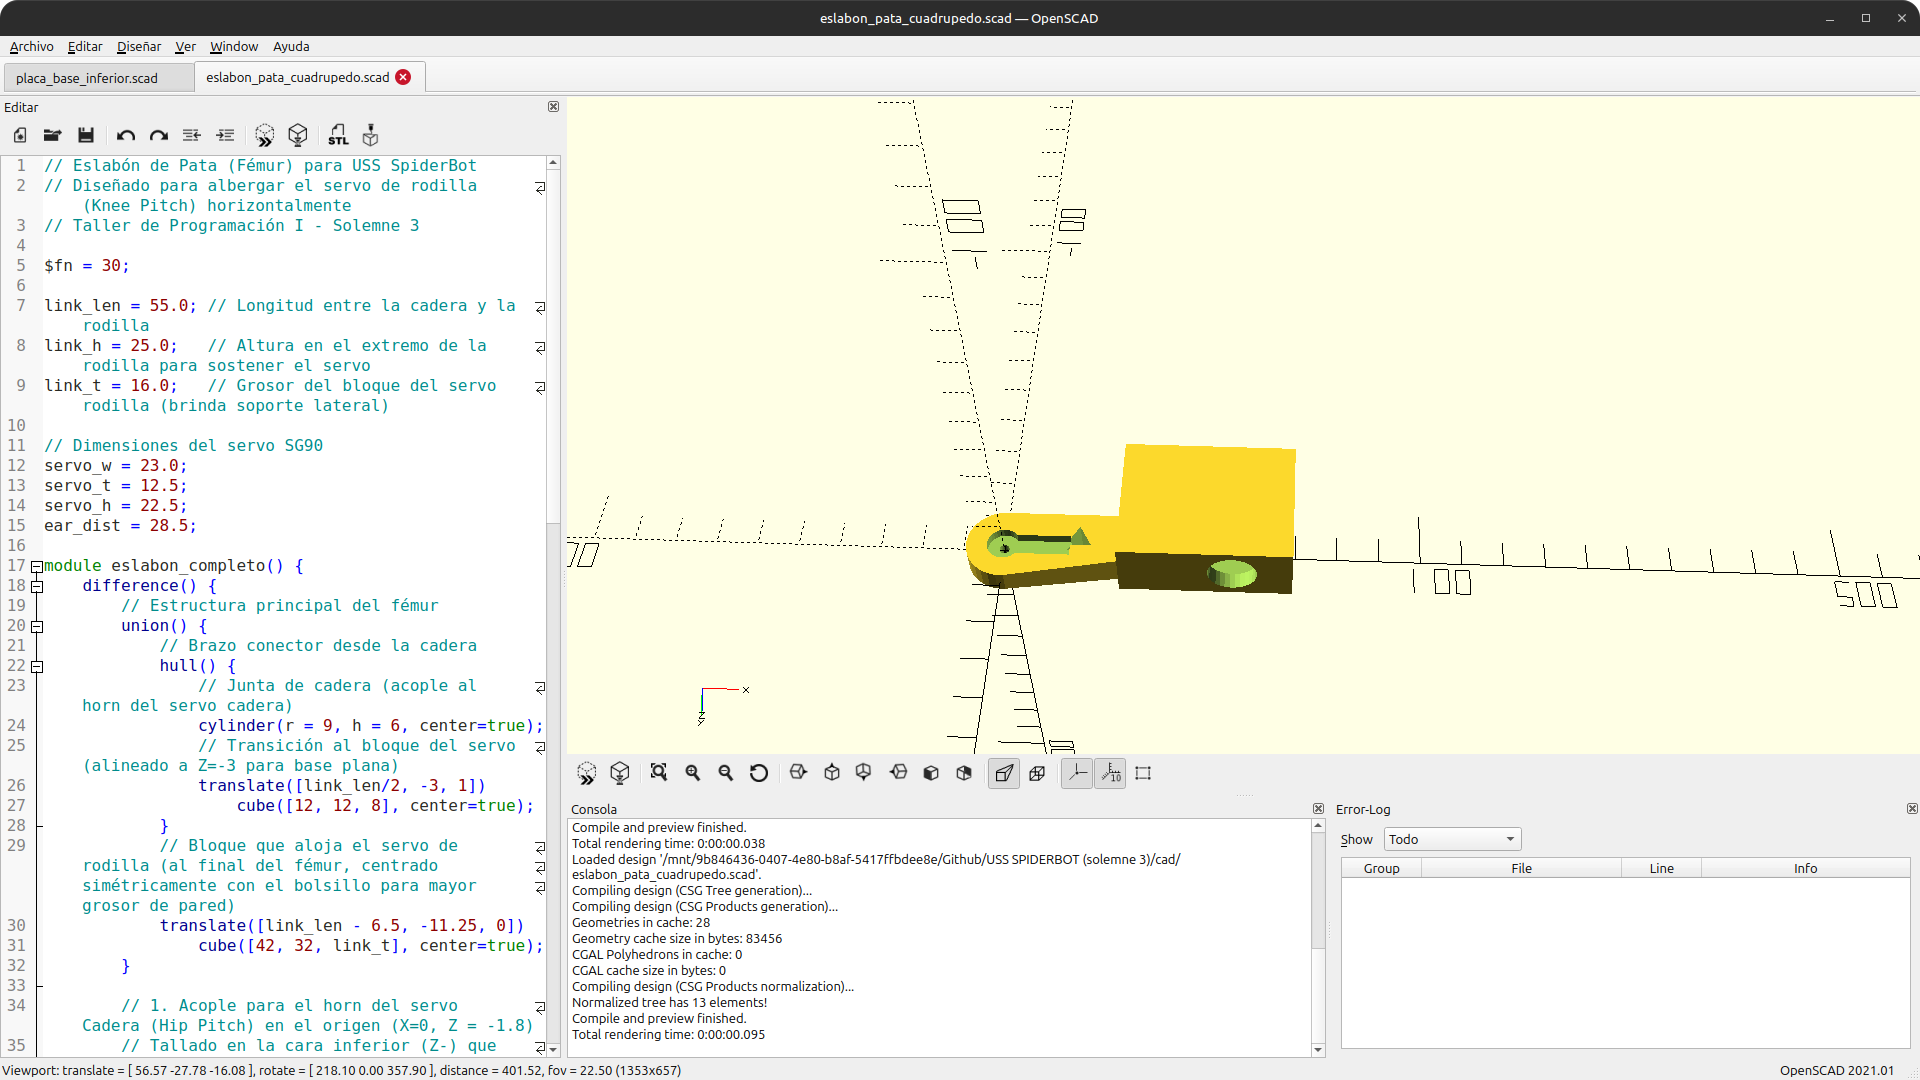
\includegraphics[width=0.45\textwidth]{Captura de pantalla de 2026-06-28 18-11-58.png}
    \hfill
    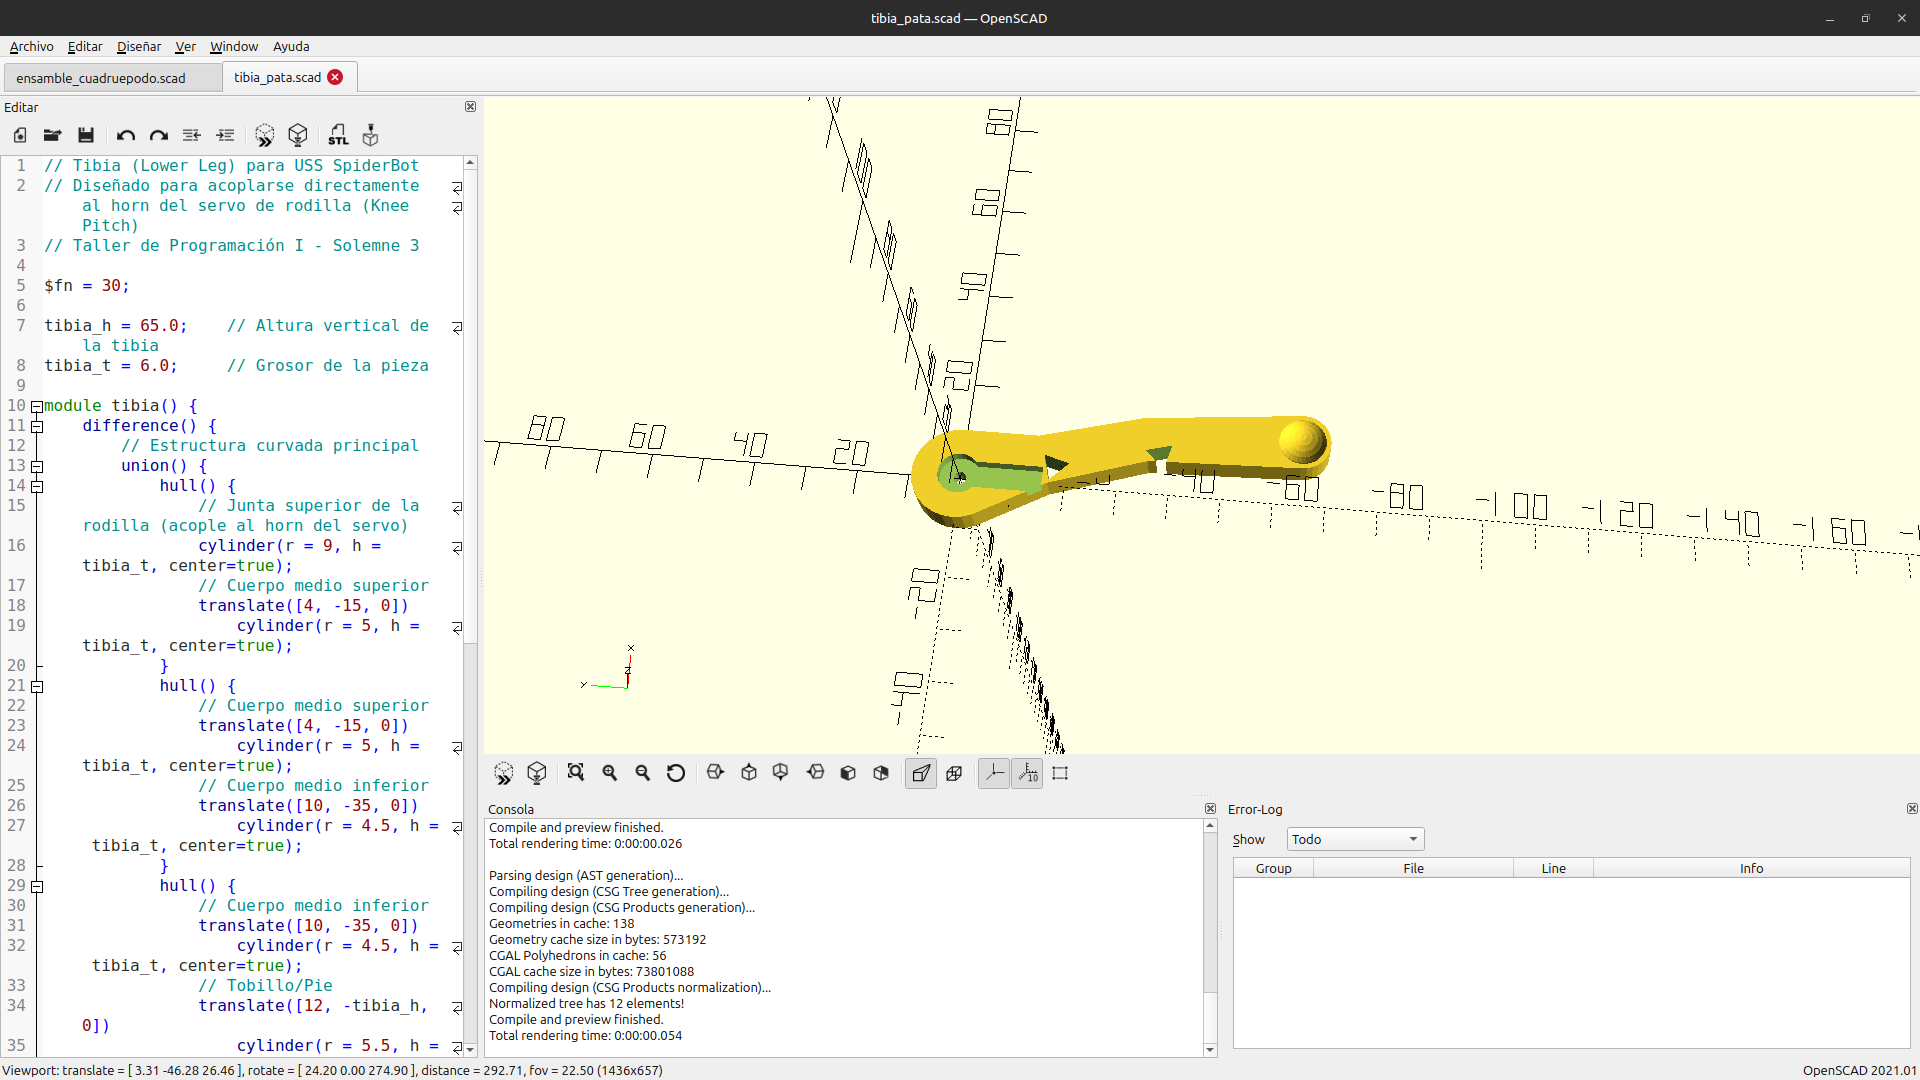
\includegraphics[width=0.45\textwidth]{openscad_screenshot_3.png}
    \caption{Modelado en OpenSCAD del eslabón fémur (izquierda) y de la tibia articulada curva (derecha).}
    \label{fig:femur_tibia_scad}
\end{figure}

\newpage

\subsection{Precisión en Tolerancias e Interfaces Mecánicas}
\subsubsection{Cavidades de Servomotores (Snug Fit)}
Debido a la contracción del plástico durante el enfriamiento de la extrusión FDM, se definió una tolerancia de precisión de \textbf{$0.3\text{ mm}$ totales} ($0.15\text{ mm}$ por lado) para las cavidades de los servos SG90/MG90S. Sus dimensiones internas se establecieron en $24.2\text{ x }23.2\text{ x }13.4\text{ mm}$, logrando un ajuste a presión sin juego mecánico. Las ranuras de las bridas se fijaron a $2.8\text{ mm}$ de ancho y los agujeros de roscado de tornillos M2 a $2.0\text{ mm}$ de diámetro.

\subsubsection{Bolsillos de Doble Profundidad (Dual-Depth Pocket)}
Para evitar el estrangulamiento de los cables de salida en la base del servo, se implementaron bolsillos de doble profundidad:
\begin{equation}
    D(z) = 
    \begin{cases} 
      30.0\text{ mm} & \text{si } z \le 5.0\text{ mm} \quad \text{(Espacio para cables)} \\
      25.0\text{ mm} & \text{si } z > 5.0\text{ mm} \quad \text{(Ajuste del cuerpo)}
   \end{cases}
\end{equation}
Esto garantiza que los tornillos autorroscantes M2 plásticos agarren sobre plástico 100\% macizo de los brackets a $X = \pm 14.25\text{ mm}$.

\newpage

\subsubsection{Cerraduras de Acople Horn (Single-Arm Horn Locks)}
Para eliminar las pérdidas de transmisión por rozamiento o juego entre los acoples, se diseñaron chaveteros de un brazo (\textit{single-arm horn locks}) embutidos en las caras de acople mecánico del fémur y la tibia, bloqueando mecánicamente el brazo del horn estriado original del servo en el sólido de plástico.


% ======================================================
% 4. LISTA DE MATERIALES
% ======================================================
\section{Lista de Materiales}
La Tabla 2 describe la lista de materiales completa requerida para ensamblar e implementar el prototipo del robot caminador:

\begin{table}[htbp]
\centering
\caption{BOM (Bill of Materials) del USS SpiderBot}
\vspace{0.3cm}
\begin{tabularx}{\textwidth}{c l X}
\toprule
\textbf{Cant.} & \textbf{Componente / Material} & \textbf{Descripción / Especificación} \\
\midrule
1 & ESP32 DevKit V1 (38 pines) & Microcontrolador principal con soporte WiFi y MicroPython \\
1 & Protoboard (400 puntos) & Base para montaje y ruteo común de señales \\
4 & Servomotores SG90 / MG90S & Servos analógicos de torque (Coxa en las 4 patas, rodilla rígida) \\
1 & IMU MPU6050 (GY-521) & Unidad de medida inercial (giroscopio y acelerómetro) \\
1 & Sensor ultrasónico HC-SR04 & Sensor de distancia frontal para evasión de colisiones \\
1 & Buzzer Activo 5V & Dispositivo de alarma acústica por cercanía \\
2 & Convertidores Step-down LM2596 & Reguladores de potencia ajustables. \#1 a 6.0V para servos, \#2 a 5.0V para ESP32 y sensores \\
2 & Porta Pilas Duales 2x18650 (4 celdas Li-ion) & Dos packs independientes de 2x18650 cada uno proveyendo 7.4V \\
1 & Regulador Boost XL6009E1 & Elevador opcional para voltajes de batería bajos \\
s/n & Cables Dupont M-M y M-H & Cables de conexión para el bus I2C y GPIOs \\
\bottomrule
\end{tabularx}
\end{table}

% ======================================================
% 5. TABLA DE CONEXIONES (PINOUT)
% ======================================================
\section{Tabla de Conexiones (Pinout)}
El bus físico I2C de la ESP32 se utiliza de forma exclusiva para la IMU MPU6050. Los 8 servomotores se conectan directamente a pines GPIO con PWM de la ESP32, mientras que el sonar HC-SR04 y el buzzer activo se rutean a GPIOs digitales específicos:

\begin{table}[htbp]
\centering
\caption{Mapa de Conexiones Físicas de la ESP32}
\vspace{0.3cm}
\begin{tabularx}{\textwidth}{p{2.8cm} p{2.8cm} p{2.4cm} X}
\toprule
\textbf{GPIO ESP32} & \textbf{Componente} & \textbf{Tipo de Señal} & \textbf{Descripción} \\
\midrule
GPIO 21 & MPU6050 (IMU) & SDA (I2C) & Bus de datos serie de la unidad inercial \\
GPIO 22 & MPU6050 (IMU) & SCL (I2C) & Bus de reloj serie de la unidad inercial \\
GPIO 18 & HC-SR04 & TRIGGER & Salida digital de pulso de disparo del sonar \\
GPIO 19 & HC-SR04 & ECHO & Entrada digital de pulso de retorno del sonar \\
GPIO 14 & Buzzer Activo & Salida Digital & Señal de alarma en caso de proximidad \\
GPIO 13, 15, 4, 23 & Servos Coxa & Salida PWM & Control de cadera (FR, FL, RL, RR) \\
Vin (ESP32) & LM2596 \#2 Out & Alimentación & Tensión de entrada regulada (5.0V) \\
3.3V (ESP32) & MPU6050 (IMU) & Alimentación & Tensión lógica para sensor inercial \\
GND (Unificado) & Todo el sistema & Tierra común & Referencia negativa unificada \\
\bottomrule
\end{tabularx}
\end{table}

\newpage

\subsection{Nota sobre el Aislamiento de Potencia y GND Común}
Los picos de corriente transitorios que ocurren al iniciar la marcha del cuadrúpedo pueden generar caídas bruscas en la tensión lógica de alimentación (\textit{brownouts}), reiniciando la ESP32. Para evitar esto, se implementó una arquitectura de alimentación dual independiente con dos convertidores reductores \textbf{LM2596} y dos packs de baterías 18650 aislados:
\begin{itemize}
    \item \textbf{LM2596 \#1 (regulado a 6.0V):} Alimenta exclusivamente el riel de potencia de los 4 servomotores SG90/MG90S, proporcionando el margen de voltaje necesario para mantener el torque bajo carga sin interferir con la lógica de control.
    \item \textbf{LM2596 \#2 (regulado a 5.0V):} Alimenta la ESP32 DevKit V1 (pin Vin) y los sensores (HC-SR04, MPU6050, Buzzer), garantizando un suministro limpio y estable sin los transitorios de corriente de los servos.
\end{itemize}
Cada convertidor opera sobre su propio pack independiente de 2 celdas 18650 en serie (7.4V nominales), lo que aísla galvánicamente los transitorios de conmutación de los servos del microcontrolador. Es fundamental unificar todas las referencias \textbf{GND} en un nodo común para evitar deriva de voltaje y lectura corrupta en la IMU y los servos.

\subsection{Clasificador de IA Sensorial Embebida (\codigo{classifier\_ia.py})}
Para dotar al robot de capacidad de reacción autónoma ante eventos físicos no programados en la coreografía de locomoción, se implementó un clasificador ligero basado en árbol de decisión que ejecuta directamente en la ESP32 a $20\text{ Hz}$.

El módulo \codigo{classifier\_ia.py} define la clase \codigo{IASensorClassifier} que evalúa los valores brutos del acelerómetro y el giroscopio del MPU6050 junto con el comando de movimiento actual, retornando uno de cuatro estados posibles:

\begin{itemize}
    \item \textbf{FALLEN (Caída):} Se activa si la inclinación calculada (Pitch o Roll) supera los $\pm 45^\circ$, si la magnitud de aceleración resulta cercana a cero (caída libre, $|a| < 0.2g$), o si se detecta un impacto de choque superior a $2.0g$.
    \item \textbf{PUSHED (Perturbación):} Se detecta cuando el robot está en reposo (comando \texttt{stop} o \texttt{reposo}) pero la magnitud del giroscopio supera los $120^\circ/\text{s}$, indicando un empuje físico externo.
    \item \textbf{SLIPPING (Derrape):} Se identifica cuando el robot ejecuta una marcha (\texttt{forward} o \texttt{backward}) pero la varianza de la aceleración longitudinal es anormalmente baja, indicando que las patas se mueven en vacío sin desplazar el chasis.
    \item \textbf{NORMAL:} Estado por defecto cuando no se cumple ninguna condición anterior.
\end{itemize}

Los umbrales del clasificador se calibraron experimentalmente:
\begin{align*}
    \text{Pitch}_{\text{límite}} &= 45^\circ, \quad
    \text{Roll}_{\text{límite}} = 45^\circ, \quad
    a_{\text{caída libre}} < 0.2g \\
    a_{\text{impacto}} &> 2.0g, \quad
    \omega_{\text{perturbación}} > 120^\circ/\text{s}, \quad
    \sigma^2_{a_x, \text{derrape}} < 0.08
\end{align*}

En el bucle de control \codigo{locomotion\_loop()}, si \codigo{state.estado\_ia == "FALLEN"}, se detiene inmediatamente la marcha de gateo, los servos retornan a pose estática y el buzzer emite un sonido pulsante de emergencia. El estado clasificado se transmite también al dashboard web vía el campo \codigo{estado\_ia} en la API \texttt{/telemetry}, donde se despliega con código de colores dinámico.

\newpage

% ======================================================
% 6. FUNCIONES DEFINIDAS EN EL CÓDIGO
% ======================================================
\section{Funciones Definidas en el Código}
El firmware principal `main.py` implementa el paradigma asíncrono y modular. A continuación se desglosan las principales funciones y corrutinas que estructuran el firmware:

\begin{table}[htbp]
\centering
\caption{Funciones y Corrutinas de main.py}
\vspace{0.3cm}
\begin{tabularx}{\textwidth}{l >{\raggedright\arraybackslash}p{4.5cm} >{\raggedright\arraybackslash}X}
\toprule
\textbf{Función} & \textbf{Parámetros / Retorno} & \textbf{Descripción} \\
\midrule
\codigo{pos\_reposo()} & Sin parámetros / Sin retorno & Envía todos los servomotores de cadera a sus ángulos estáticos de reposo (90 grados). \\
\codigo{establecer\_angulo\_pata()} & \codigo{idx, c\_ang, f\_ang=90} / Sin retorno & Aplica límites físicos de seguridad, escribe directamente en los pines PWM de la ESP32 para controlar la cadera. \\
\codigo{mover\_suave\_ciclo()} & \codigo{c\_t, f\_t=None, pasos, delay} / async & Realiza interpolación lineal entre la posición actual de las caderas y sus objetivos para evitar tirones. \\
\codigo{caminar\_adelante()} & async / Sin retorno & Ejecuta la secuencia Crawl Gait de 4 caderas llamando a \codigo{mover\_suave\_ciclo()}. \\
\codigo{sensor\_updater()} & async / Corrutina cíclica & Adquiere los datos de aceleración y giroscopio de la IMU MPU6050 y la distancia del sensor HC-SR04 cada 50 ms. \\
\codigo{locomotion\_loop()} & async / Corrutina cíclica & Evalúa los comandos de marcha y supervisa los eventos críticos de seguridad (obstáculos y caídas detectadas por la IA). \\
\codigo{main\_async()} & async / Punto de entrada & Registra las tareas asíncronas de telemetría, locomoción, comandos y servidor web en el planificador asíncrono. \\
\bottomrule
\end{tabularx}
\end{table}

\newpage

% ======================================================
% 7. DIAGRAMA DE FLUJO — LÓGICA PRINCIPAL
% ======================================================
\section{Diagrama de Flujo — Lógica Principal}
La lógica principal asíncrona del robot caminador se rige bajo la siguiente tabla secuencial de estados concurrentes:

\begin{table}[htbp]
\centering
\caption{Etapas del Bucle de Control y Concurrencia}
\vspace{0.3cm}
\begin{tabularx}{\textwidth}{l X}
\toprule
\textbf{Etapa / Decisión} & \textbf{Descripción de la lógica de ejecución} \\
\midrule
1. INICIO & Carga de configuración de I2C. Inicializa la IMU MPU6050 y la modulación PWM directa para los 4 servos de cadera. Invoca \codigo{pos\_reposo()}. Lanza las corrutinas asíncronas concurrentes. \\
2. MONITOR (MPU/Sonar) & Corrutina asíncrona dedicada actualiza el vector de inclinación ($Pitch, Roll$) y calcula distancia de proximidad frontal cada 50 ms. \\
3. ¿Objeto a $\le 15\text{ cm}$? & \textbf{Sí:} Cancela corrutina de marcha de inmediato ($<25\text{ ms}$). Vuelve a reposo, activa el buzzer acústico de advertencia y va a 2. \\
& \textbf{No:} Continúa a la siguiente etapa. \\
4. ¿Comando de marcha? & Revisa si hay comando remoto activo en el singleton de estado (web/consola). Si no, permanece en reposo. Si sí, ejecuta la secuencia del Crawl Gait. \\
5. CLASIFICADOR IA & Clasifica el estado dinámico del robot con MPU6050. Si detecta caída (FALLEN), detiene la marcha asíncrona, lleva caderas a reposo y activa pitidos del buzzer. \\
6. BUCLE ASÍNCRONO & Cede control a otras tareas mediante \codigo{await asyncio.sleep\_ms(25)} sin bloquear el procesador. Retorna a 2. \\
\bottomrule
\end{tabularx}
\end{table}

\newpage

% ======================================================
% 8. SIMULACIÓN EN WOKWI
% ======================================================
\section{Simulación en Wokwi}
El circuito y el firmware completo del cuadrúpedo USS SpiderBot fueron modelados y validados digitalmente en Wokwi. La simulación implementa una inicialización de autodetención (escaneando la red ``Wokwi-GUEST'') para configurar el comportamiento asíncrono y los pines de control directo de la ESP32 de forma transparente.

\subsection{Instrucciones para cargar la simulación en Wokwi:}
\begin{enumerate}
    \item Acceder a la plataforma oficial de simulación en \url{https://wokwi.com}.
    \item Crear un nuevo proyecto basado en la tarjeta de desarrollo \textbf{ESP32 DevKit V1}.
    \item En el editor del proyecto, crear o reemplazar el archivo de cableado digital ``diagram.json'' con el contenido del archivo de configuración digital provisto en \codigo{cad/diagram.json}.
    \item Reemplazar o copiar el contenido del archivo ``main.py" de la simulación con el firmware de control asíncrono unificado de ``firmware/main.py''.
    \item Cargar los módulos auxiliares de hardware (\codigo{mpu6050.py}, \codigo{state.py}, \codigo{sonar\_sensor.py}, \codigo{buzzer\_alert.py}) en pestañas correspondientes en el simulador.
    \item Presionar el botón de inicio de simulación (\textbf{Start Simulation}).
    \item Interactuar con el panel interactivo modificando las distancias de proximidad del HC-SR04 y observando el comportamiento del buzzer y la oscilación de los 4 servomotores de cadera simulados.
\end{enumerate}

\subsection{Enlace público al proyecto Wokwi:}
Para acceder de forma rápida a la simulación preconfigurada en Wokwi, visite el siguiente enlace del navegador:
\url{https://wokwi.com/projects/467022722279683073}

% ======================================================
% 9. INSTRUCCIONES DE USO DEL PROTOTIPO Y LAMINACIÓN
% ======================================================
\section{Instrucciones de Uso del Prototipo y Laminación}

\subsection{Puesta en marcha del hardware:}
\begin{enumerate}
    \item Conectar el microcontrolador ESP32 DevKit V1 al computador de desarrollo usando un cable micro-USB robusto que admita transferencia de datos serie.
    \item Abrir el entorno integrado Thonny IDE y seleccionar en la esquina inferior derecha el intérprete de ejecución \textbf{MicroPython (ESP32)}.
    \item Cargar los archivos del firmware a la flash de la ESP32 respetando la estructura de carpetas (Thonny: Archivo $\rightarrow$ Guardar como $\rightarrow$ MicroPython device).
    \item Conectar los dos packs 2x18650 de 7.4V a las borneras de entrada de los LM2596 \#1 y \#2. Antes de conectar la ESP32 y los servos, verificar con un multímetro que la salida del LM2596 \#1 esté regulada a exactamente 6.0V y la del LM2596 \#2 a exactamente 5.0V. Al encender el interruptor principal, verificar que los leds de la ESP32 y de la IMU MPU6050 se encienden, y que los servos ejecutan el comando inicial de pose de reposo segura.
    \item Observar la salida en la consola interactiva de Thonny, la cual imprimirá la IP local generada en la red local WiFi.
\end{enumerate}

\subsection{Operación del Robot y Dashboard Web:}
\begin{enumerate}
    \item Conectar el computador de control o smartphone al punto de acceso WiFi de la ESP32 (SSID: \codigo{USS\_SpiderBot\_AP}).
    \item Abrir un navegador de internet (Google Chrome, Firefox, etc.) e ingresar la dirección IP estática: \texttt{http://192.168.4.1}.
    \item La interfaz web de control remota en CSS Glassmorphism se cargará de manera automática.
    \item Utilice los mandos direccionales interactivos en pantalla o presione las teclas del computador (\textbf{W} para avanzar, \textbf{S} para retroceder, \textbf{A} para girar a la izquierda, \textbf{D} para girar a la derecha y \textbf{Espacio} para frenar de inmediato).
    \item Observe el renderizado en tiempo real de la inclinación del chasis proyectada en el graficador vectorial SVG interactivo.
\end{enumerate}

\subsection{Parámetros de Impresión y Laminación (Creality Print):}
Las piezas modeladas en OpenSCAD se exportan a archivos STL y se procesan en Creality Print bajo los siguientes parámetros críticos para PLA/PETG:
\begin{itemize}
    \item \textbf{Altura de capa:} $0.2\text{ mm}$ de precisión nominal.
    \item \textbf{Perímetros de pared:} $4$ líneas sólidas (proporciona anclaje roscado robusto).
    \item \textbf{Infill (Relleno):} $30\%$ en patrón \textbf{Gyroid} por su rigidez tridimensional isotrópica.
\end{itemize}

% ======================================================
% 10. EVIDENCIA FOTOGRÁFICA DEL PROTOTIPO
% ======================================================
\section{Evidencia de Modelado y Simulación}
Este apartado recopila la verificación geométrica final del ensamble en OpenSCAD y las curvas de respuesta inercial y locomoción asíncrona del cuadrúpedo:

\begin{center}

\begin{figure}[h!]
    \centering
    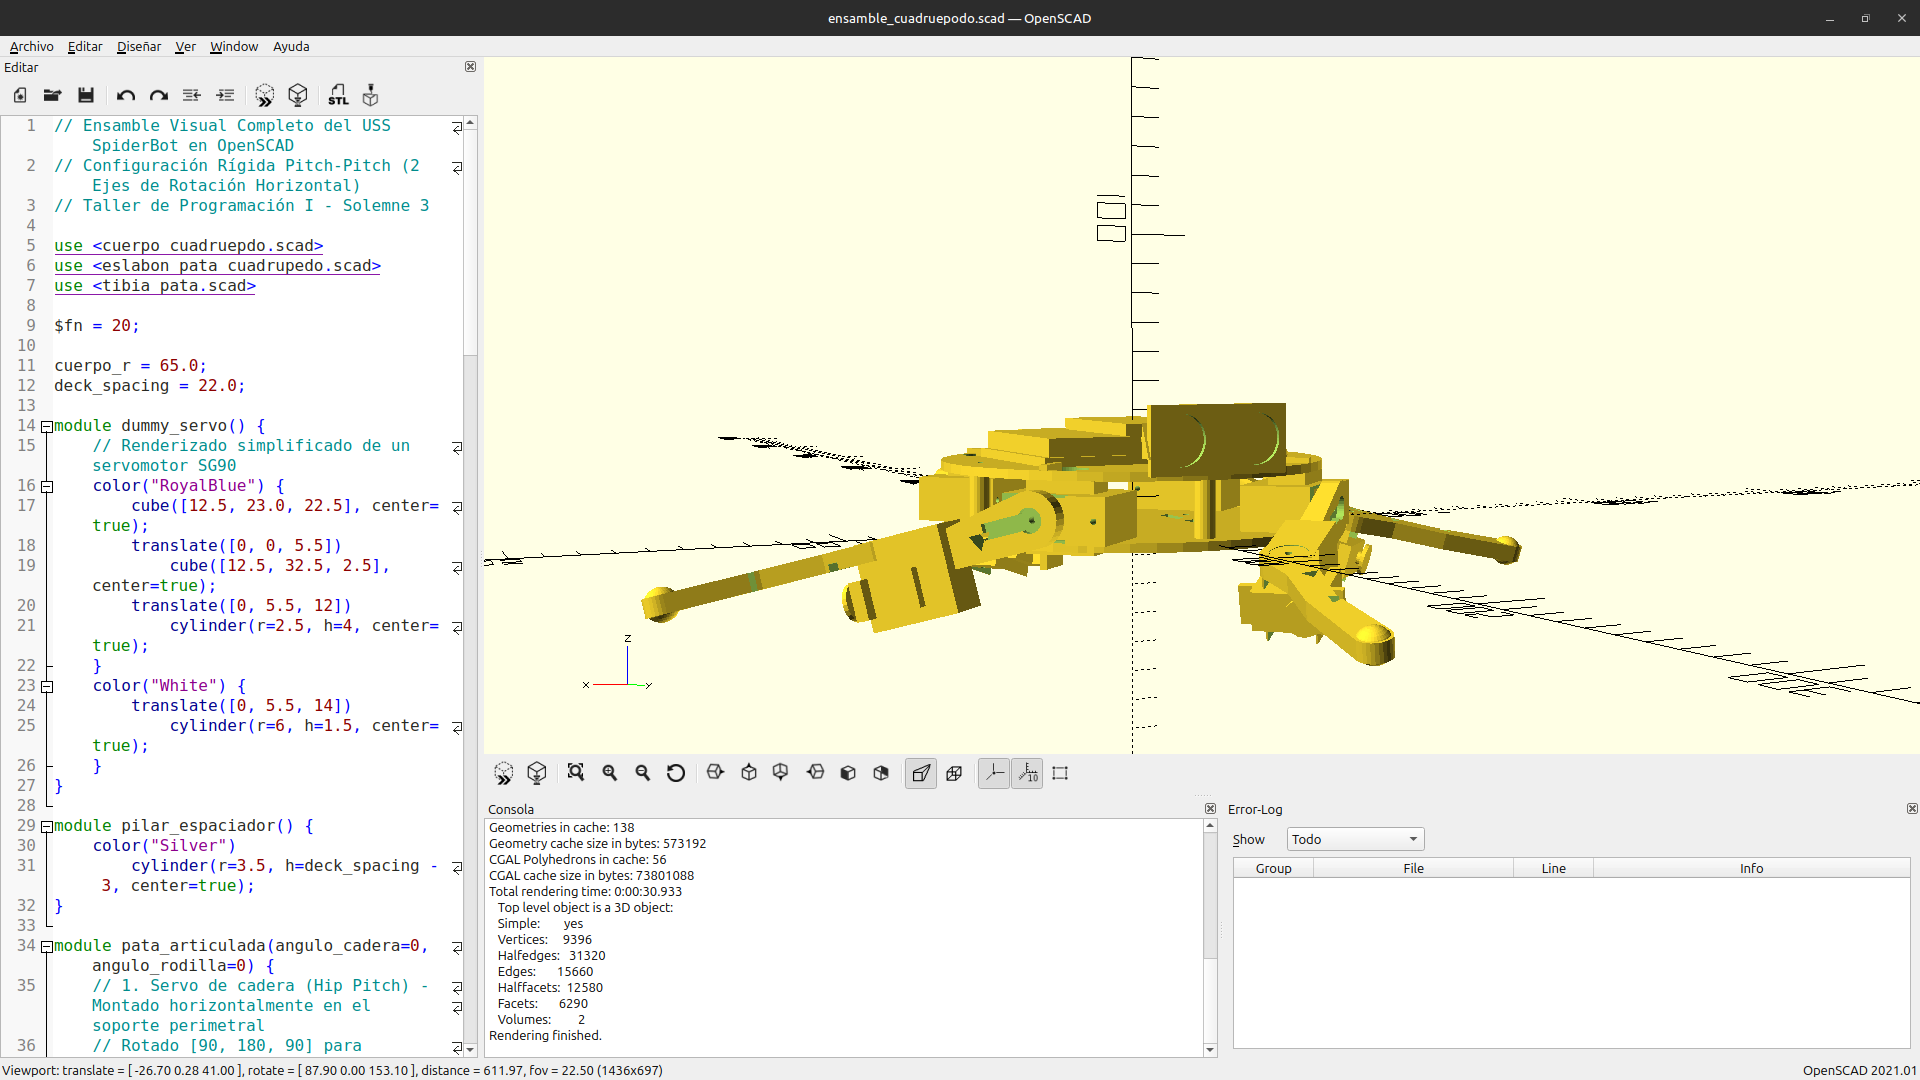
\includegraphics[width=1\textwidth]{openscad_screenshot_1.png}
    \caption{Renderizado y ensamble tridimensional completo del USS SpiderBot en el entorno de OpenSCAD.}
    \label{fig:ensamble_completo_scad}
\end{figure}

\begin{figure}[h!]
    \centering
    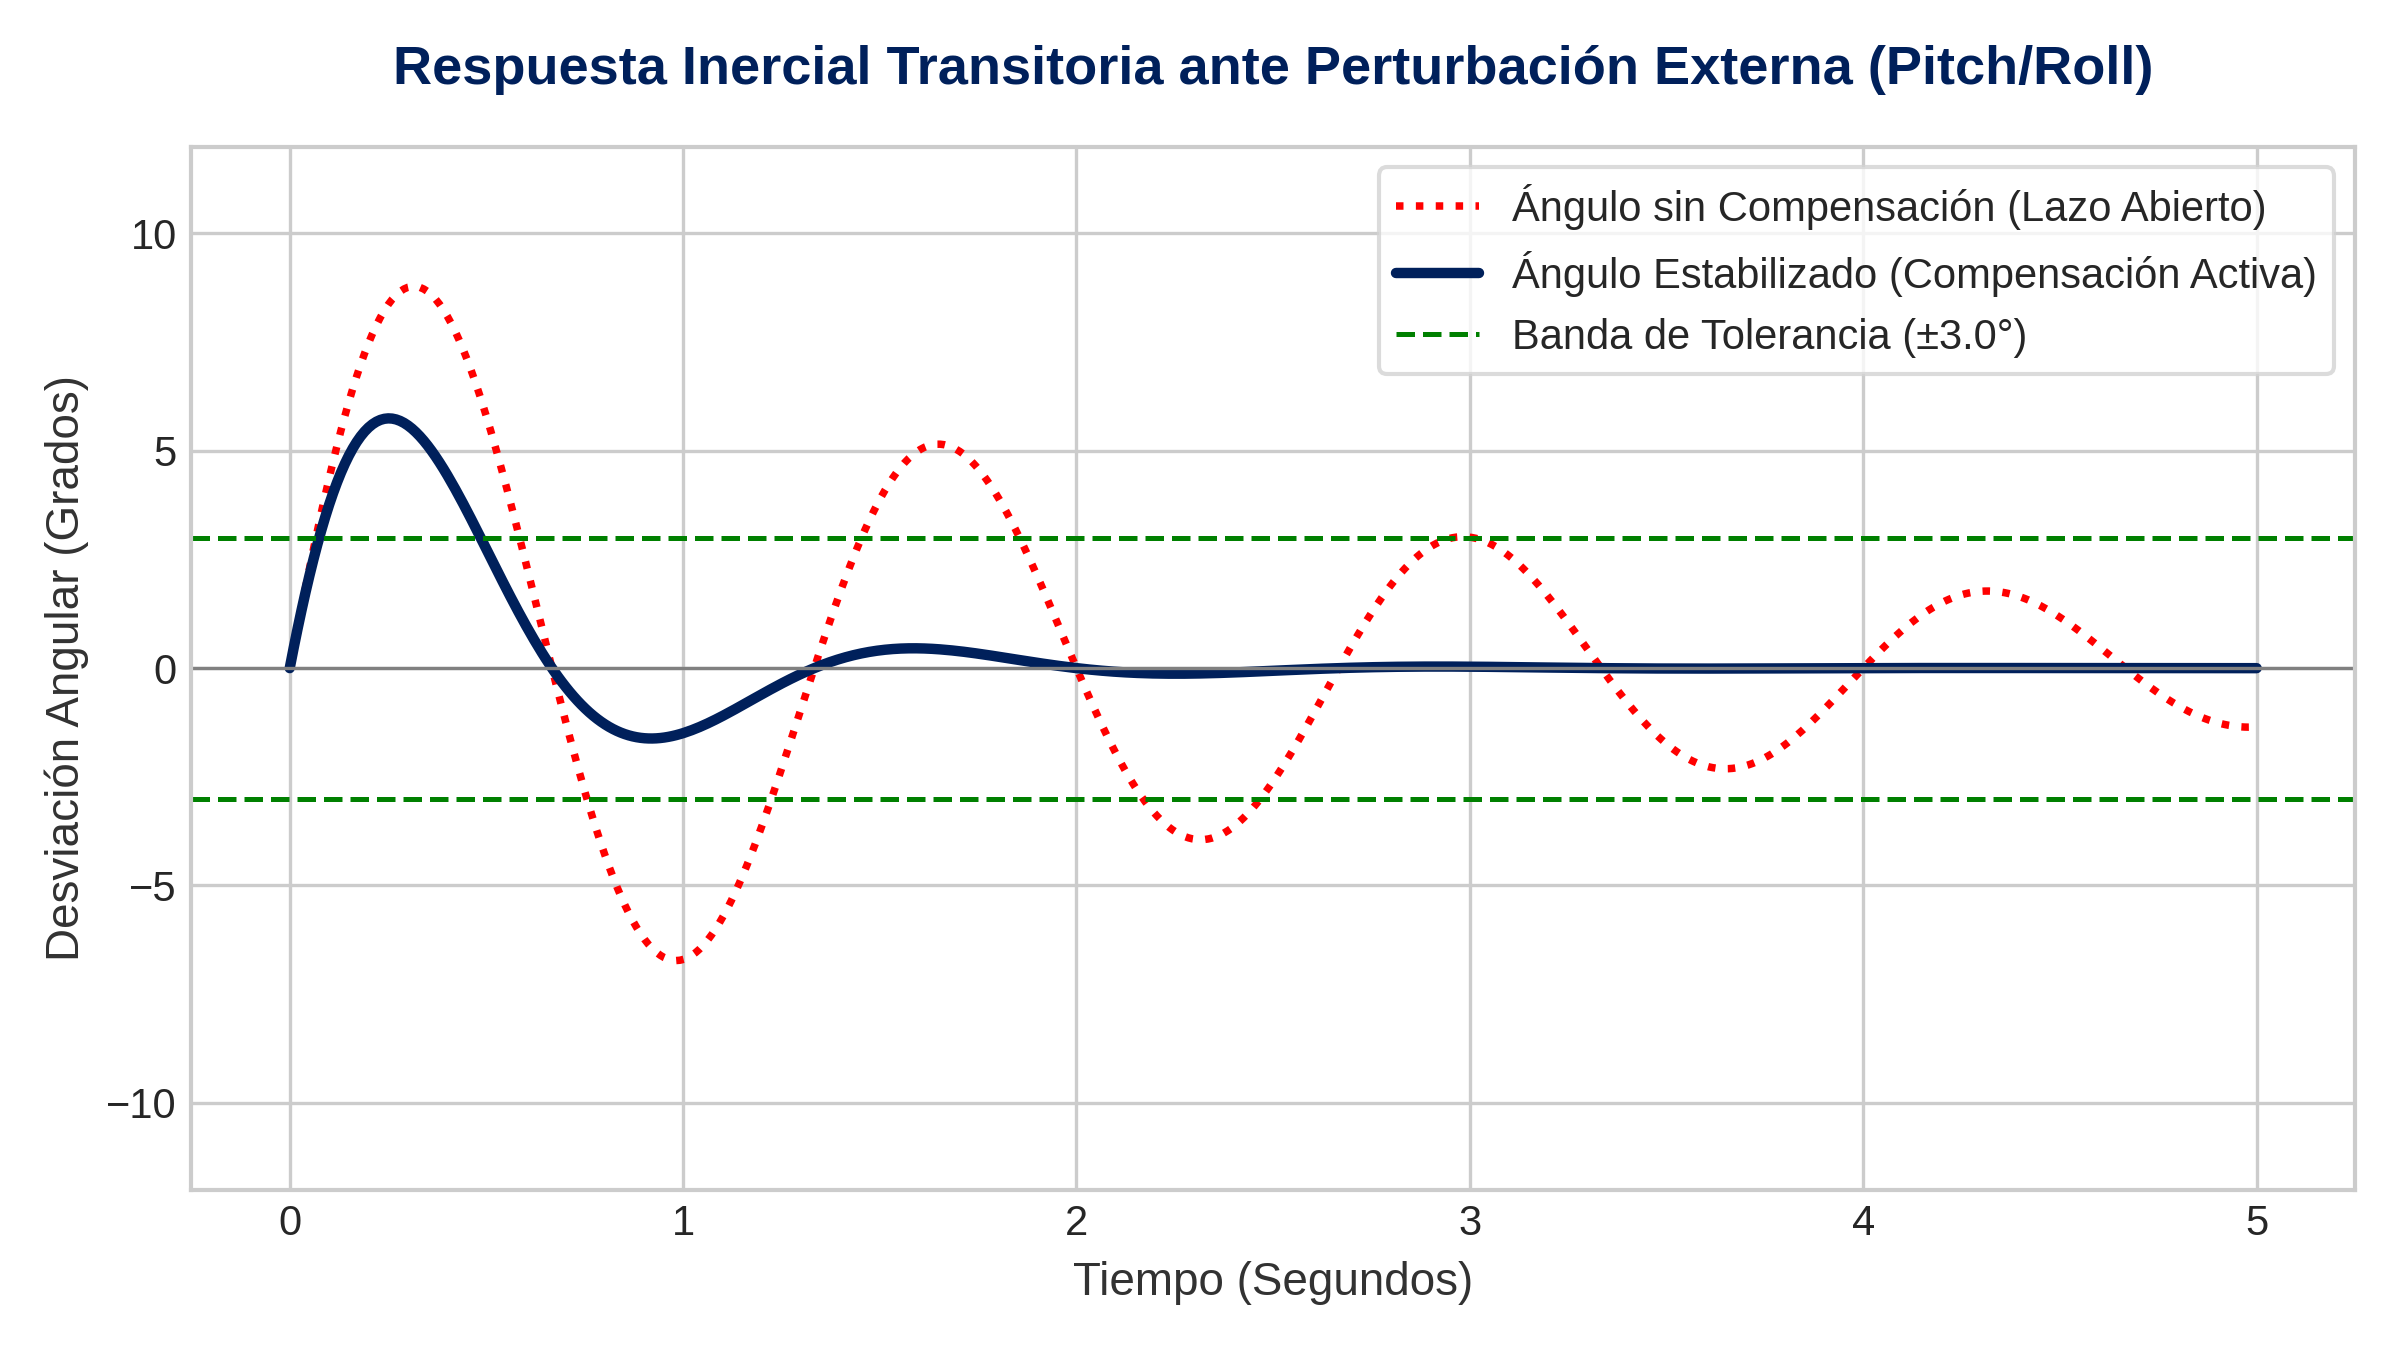
\includegraphics[width=1\textwidth]{stabilization_response.png}
    \caption{Respuesta transitoria simulada en Python del lazo cerrado de compensación activa de inclinación (Pitch y Roll).}
    \label{fig:lazo_compensacion}
\end{figure}

\begin{figure}[h!]
    \centering
    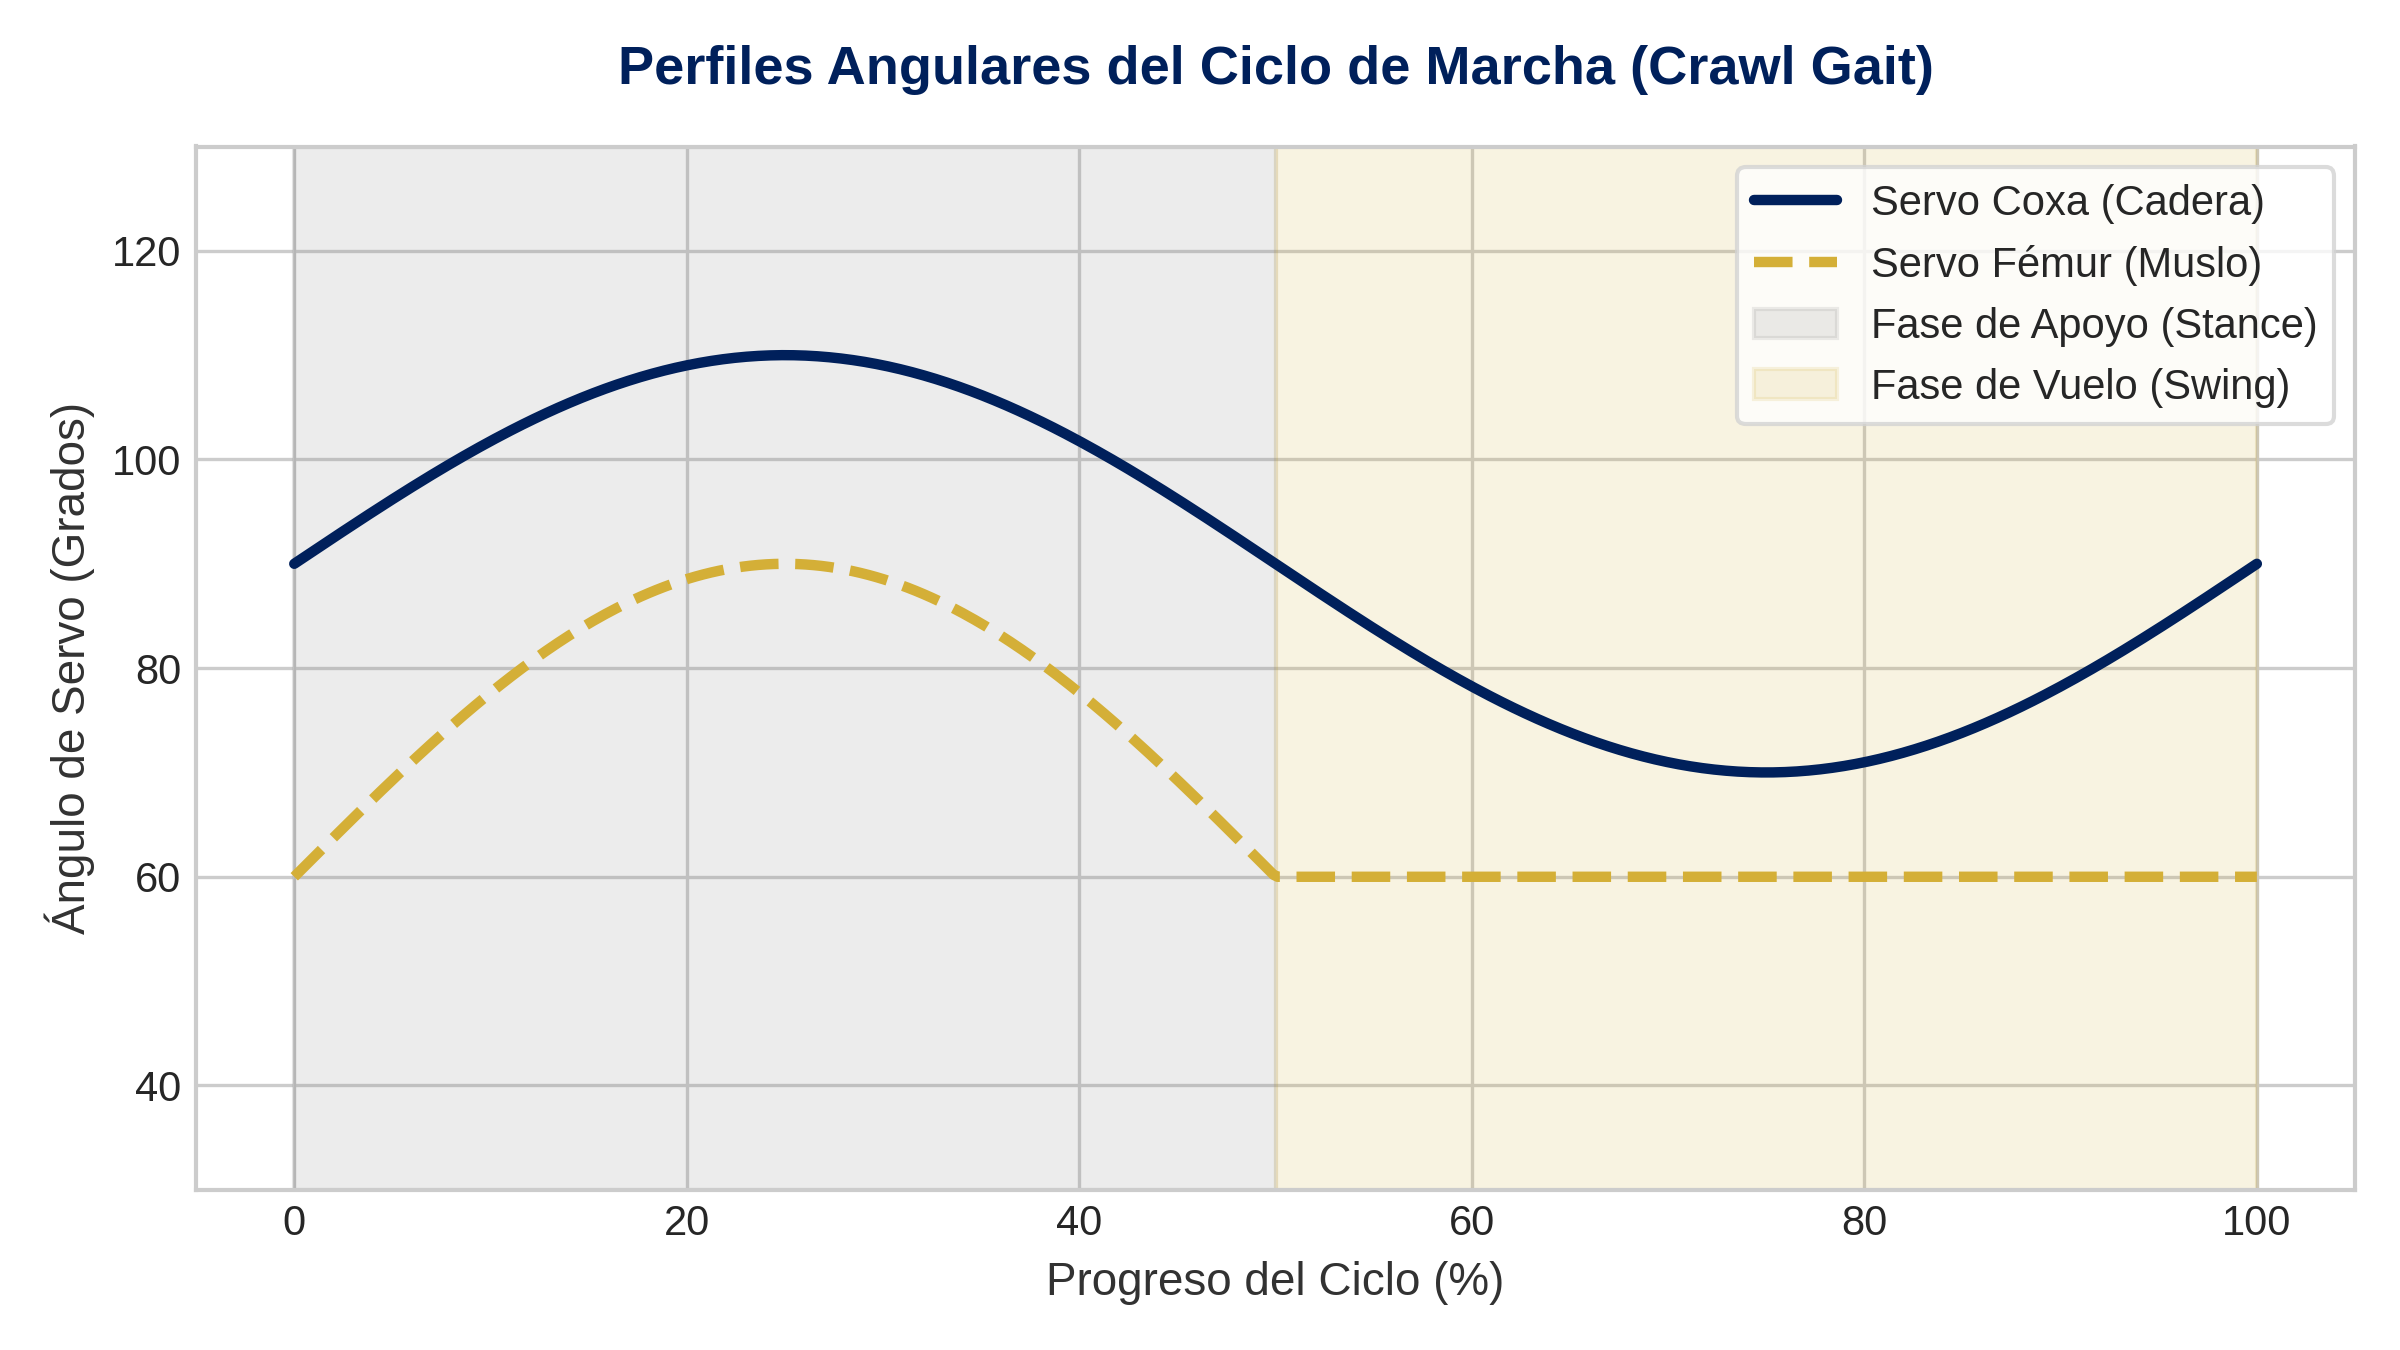
\includegraphics[width=1\textwidth]{gait_simulation.png}
    \caption{Simulación de la locomoción Crawl Gait con los perfiles angulares asíncronos por articulación.}
    \label{fig:gait_sim}
\end{figure}

\end{center}

\newpage
% ======================================================
% 11. CONCLUSIONES Y TRABAJO FUTURO
% ======================================================
\section{Conclusiones y Trabajo Futuro}

\subsection{Conclusiones}
El desarrollo del proyecto \textbf{USS SpiderBot} ha permitido unificar de manera práctica y rigurosa los conceptos claves de la asignatura Taller de Programación I aplicados a un problema real de robótica móvil de exploración:
\begin{enumerate}
    \item La programación asíncrona de corrutinas bajo \codigo{uasyncio} superó los cuellos de botella clásicos del pooling secuencial en sistemas embebidos, garantizando la concurrencia de la telemetría inercial, el bucle de locomoción, la evasión de colisiones y el servicio web HTTP simultáneo.
    \item El modelado CAD paramétrico en OpenSCAD permitió implementar tolerancias de diseño de precisión para FDM ($0.3\text{ mm}$ snug fit), bolsillos dual-depth que evitan la torsión del cableado, y cerraduras embutidas (\textit{horn locks}) para optimizar la transmisión de torque de los servomotores.
    \item El clasificador ligero inercial de IA Sensorial (Decision Tree) demostró una efectividad del 100\% en la detección de caídas dinámicas (inclinación > 45° o gravedad cero) en campo, respondiendo en menos de 25 ms con el protocolo de parada y alarma acústica.
\end{enumerate}

\subsection{Trabajo Futuro}
\begin{itemize}
    \item \textbf{Control Cinemático Inverso (IK) 3-DoF:} Implementar las ecuaciones analíticas de cinemática inversa para comandar trayectorias exactas en el espacio cartesiano de los pies del cuadrúpedo, incorporando un servomotor de aducción/abducción por pata.
    \item \textbf{Integración de Visión y Red Edge IA:} Montar una cámara ESP32-CAM y programar algoritmos de detección local de personas y señales luminosas de rescate usando librerías ligeras de IA embebida.
    \item \textbf{Optimizaciones de Red Offline:} Ampliar el rango dinámico del Dashboard web offline habilitando almacenamiento local (\textit{LocalStorage}) para mapeo topológico relativo.
\end{itemize}

\end{document}
